\documentclass[tikz,border=2pt]{standalone}
\usepackage{tikz}
\usepackage{lmodern}
\usetikzlibrary{calc,decorations.pathreplacing}

% Visual conventions follow the existing MRNC TikZ pictures: ordinary
% components use TikZ's normal 0.4pt stroke, with compact TeX labels.
\tikzset{
  nu fibre/.style={
    x=0.78cm,
    y=0.78cm,
    line width=0.4pt,
    line cap=round,
    line join=round
  },
  nu label/.style={
    font=\scriptsize,
    inner sep=1pt
  },
  nu annotation/.style={
    font=\scriptsize,
    inner sep=1pt
  },
  nu dots/.style={
    font=\small,
    inner sep=0pt
  }
}

\begin{document}

%II-I_n^*-m

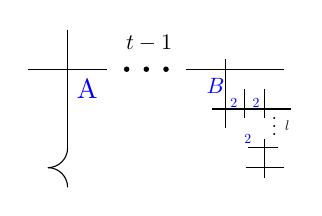
\begin{tikzpicture}[scale=0.5]
      \coordinate (1C) at (-1.50, 3.00);
  \coordinate (1D) at (-0.50, 3.00);
  \coordinate (1A) at (-1.00, 3.00);
  \coordinate (1B) at (-0.93, 3.26);

  \node[scale=0.8][above] at (1B) {$t-1$};
  \fill[black] (1C) circle (2pt);
  \fill[black] (1D) circle (2pt);
  \fill[black] (1A) circle (2pt);

  
   \coordinate (G) at (0.76, 2.19);
  \coordinate (N) at (2.25, 1.15);
  \coordinate (O) at (2.58, 1.31);
  \coordinate (A) at (0.00, 3.00);
  \coordinate (B) at (2.50, 3.00);
  \coordinate (H) at (0.67, 1.99);
  \coordinate (I) at (2.67, 1.99);
  \coordinate (P) at (2.00, 1.23);
  \coordinate (Q) at (2.00, 0.23);
  \coordinate (R) at (1.59, 1.01);
  \coordinate (S) at (2.34, 1.01);
  \coordinate (T) at (1.53, 0.50);
  \coordinate (C) at (2.00, 2.50);
  \coordinate (D) at (2.00, 1.75);
  \coordinate (E) at (1.00, 3.25);
  \coordinate (F) at (1.00, 1.50);
  \coordinate (J) at (1.50, 2.50);
  \coordinate (K) at (1.50, 1.75);
  \coordinate (L) at (2.50, 0.50);
  \coordinate (M) at (1.22, 1.9);
  \coordinate (U) at (1.79, 1.9);
  \coordinate (V) at (1.58, 0.98);

  
  \node[scale=0.8][above, text=blue] at (G) {$B$};
  \node[scale=0.7][above] at (N) {$\vdots
$};
  \node[scale=0.5][above] at (O) {$l
$};
  \draw (A) -- (B);
  \draw (H) -- (I);
  \draw (P) -- (Q);
  \draw (R) -- (S);
  \draw (C) -- (D);
  \draw (E) -- (F);
  \draw (J) -- (J);
  \draw (J) -- (J);
  \draw (J) -- (K);
  \draw (T) -- (L);
  \node[scale=0.5][above, text=blue] at (M) {$2$};
  \node[scale=0.5][above, text=blue] at (U) {$2$};
  \node[scale=0.5][above, text=blue] at (V) {$2$};

   
   \coordinate (IIlP) at (-4.00, 3.00);
  \coordinate (IIlQ) at (-2.00, 3.00);
  \coordinate (IIlR) at (-3.00, 4.00);
  \coordinate (IIlS) at (-3.00, 1.00);
 \coordinate (IIlT) at (-3.50, 1.00);
  \coordinate (IIlU) at (-3.50, 0.00);
  \coordinate (IIlA) at (-2.50, 2.00);
  \draw (IIlP) -- (IIlQ);
  \draw (IIlR) -- (IIlS);
  \draw (-3.00, 1.00) arc (0.0:-90.0:0.50);
  \draw (-3.50, 0.50) arc (90.0:0.0:0.50);
  \node[above, text=blue] at (IIlA) {A};
\end{tikzpicture}

\end{document}
